\chapter{函数列与函数项级数}

\section{一致收敛性}

我们已经知道可以用收敛数列 (或数项级数) 来表示或定义一个数. 本章将讨论怎样用函数列 (或函数项级数) 来表示 (或定义) 一个函数, 并研究这个函数所具有的性质.

\subsection{函数列及其一致收敛性}

设
\[
{f}_{1},{f}_{2},\cdots ,{f}_{n},\cdots  \tag{1}
\]
是一列定义在同一数集 \(E\) 上的函数,称为定义在 \(E\) 上的函数列. (1) 也可简单地写作
\[
\left\{  {f}_{n}\right\}  \text{ 或 }{f}_{n},n = 1,2,\cdots \text{ . }
\]
设 \({x}_{0} \in  E\) ,以 \({x}_{0}\) 代入 (1) 可得数列
\[
{f}_{1}\left( {x}_{0}\right) ,{f}_{2}\left( {x}_{0}\right) ,\cdots ,{f}_{n}\left( {x}_{0}\right) ,\cdots . \tag{2}
\]
若数列 (2) 收敛,则称函数列 (1) 在点 \({x}_{0}\) 收敛, \({x}_{0}\) 称为函数列 (1) 的收敛点. 若数列 (2) 发散,则称函数列 (1) 在点 \({x}_{0}\) 发散. 若函数列 (1) 在数集 \(D \subset  E\) 上每一点都收敛,则称 (1) 在数集 \(D\) 上收敛. 这时对 \(D\) 上每一点 \(x\) ,都有数列 \(\left\{  {{f}_{n}\left( x\right) }\right\}\) 的一个极限值与之相对应,由这个对应法则所确定的 \(D\) 上的函数,称为函数列 (1) 的极限函数. 若把此极限函数记作 \(f\) ,则有
\[
\mathop{\lim }\limits_{{n \rightarrow  \infty }}{f}_{n}\left( x\right)  = f\left( x\right) ,\;x \in  D
\]
或
\[
{f}_{n}\left( x\right)  \rightarrow  f\left( x\right) \;\left( {n \rightarrow  \infty }\right) ,\;x \in  D.
\]
函数列极限的 \(\varepsilon  - N\) 定义是: 对每一固定的 \(x \in  D\) ,任给正数 \(\varepsilon\) ,恒存在正数 \(N\) (注意:一般说来 \(N\) 值的确定与 \(\varepsilon\) 和 \(x\) 的值都有关,所以也用 \(N\left( {\varepsilon ,x}\right)\) 表示它们之间的依赖关系),使得当 \(n > N\) 时,总有
\[
\left| {{f}_{n}\left( x\right)  - f\left( x\right) }\right|  < \varepsilon .
\]
使函数列 \(\left\{  {f}_{n}\right\}\) 收敛的全体收敛点集合,称为函数列 \(\left\{  {f}_{n}\right\}\) 的收敛域.

%例 1
\begin{example}

\end{example}
设 \({f}_{n}\left( x\right)  = {x}^{n},n = 1,2,\cdots\) 为定义在 \(\left( {-\infty , + \infty }\right)\) 上的函数列,证明它的收敛域是 \(( - 1,1\rbrack\) ,且有极限函数
\[
f\left( x\right)  = \left\{  \begin{array}{ll} 0, & \left| x\right|  < 1, \\  1, & x = 1. \end{array}\right.  \tag{3}
\]
%证
\begin{proof}

\end{proof}
任给 \(\varepsilon  > 0\) (不妨设 \(\varepsilon  < 1\) ),当 \(0 < \left| x\right|  < 1\) 时,由于
\[
\left| {{f}_{n}\left( x\right)  - f\left( x\right) }\right|  = {\left| x\right| }^{n},
\]
只要取 \(N\left( {\varepsilon ,x}\right)  = \frac{\ln \varepsilon }{\ln \left| x\right| }\) ,当 \(n > N\left( {\varepsilon ,x}\right)\) 时,就有
\[
\left| {{f}_{n}\left( x\right)  - f\left( x\right) }\right|  < \varepsilon .
\]
当 \(x = 0\) 和 \(x = 1\) 时,则对任何正整数 \(n\) ,都有
\[
\left| {{f}_{n}\left( 0\right)  - f\left( 0\right) }\right|  = 0 < \varepsilon ,\;\left| {{f}_{n}\left( 1\right)  - f\left( 1\right) }\right|  = 0 < \varepsilon .
\]
这就证得 \(\left\{  {f}_{n}\right\}\) 在 \(( - 1,1\rbrack\) 上收敛,且有 (3) 式所表示的极限函数.

当 \(\left| x\right|  > 1\) 时,则有 \({\left| x\right| }^{n} \rightarrow   + \infty \left( {n \rightarrow  \infty }\right)\) ,当 \(x =  - 1\) 时,对应的数列为
\[
- 1,1, - 1,1,\cdots \text{ . }
\]
它显然是发散的. 所以函数列 \(\left\{  {x}^{n}\right\}\) 在区间 \(( - 1,1\rbrack\) 外都是发散的.

%例 2
\begin{example}

\end{example}
定义在 \(\left( {-\infty , + \infty }\right)\) 上的函数列 \({f}_{n}\left( x\right)  = \frac{\sin {nx}}{n},n = 1,2,\cdots\) . 由于对任何实数 \(x\) ,都有
\[
\left| \frac{\sin {nx}}{n}\right|  \leq  \frac{1}{n}
\]
故对任给的 \(\varepsilon  > 0\) ,只要 \(n > N = \frac{1}{\varepsilon }\) ,就有
\[
\left| {\frac{\sin {nx}}{n} - 0}\right|  < \varepsilon .
\]
所以函数列 \(\left\{  \frac{\sin {nx}}{n}\right\}\) 的收敛域为无限区间 \(\left( {-\infty , + \infty }\right)\) ,极限函数 \(f\left( x\right)  = 0\) .

对于函数列, 我们不仅要讨论它在哪些点上收敛, 而更重要的是要研究极限函数所具有的解析性质. 比如能否由函数列每项的连续性判断出极限函数的连续性. 又如极限函数的导数或积分, 是否分别是函数列每项导数或积分的极限. 对这些问题的讨论,只要求函数列在数集 \(D\) 上收敛是不够的,必须对它在 \(D\) 上的收敛性提出更高的要求才行, 这就是以下所要讨论的一致收敛性问题.

%定义  1
\begin{definition}{}{def:}

\end{definition}
设函数列 \(\left\{  {f}_{n}\right\}\) 与函数 \(f\) 定义在同一数集 \(D\) 上,若对任给的正数 \(\varepsilon\) ,总存在某一正整数 \(N\) ,使得当 \(n > N\) 时,对一切 \(x \in  D\) ,都有
\[
\left| {{f}_{n}\left( x\right)  - f\left( x\right) }\right|  < \varepsilon ,
\]
则称函数列 \(\left\{  {f}_{n}\right\}\) 在 \(D\) 上一致收敛于 \(f\) ,记作
\[
{f}_{n}\left( x\right)  \rightarrow  f\left( x\right) \left( {n \rightarrow  \infty }\right) ,\;x \in  D.
\]
由定义看到,如果函数列 \(\left\{  {f}_{n}\right\}\) 在 \(D\) 上一致收敛,那么对于所给的 \(\varepsilon\) ,不管 \(D\) 上哪一点 \(x\) ,总存在公共的 \(N\left( \varepsilon \right)\) (即 \(N\) 的选取仅与 \(\varepsilon\) 有关,与 \(x\) 的取值无关),只要 \(n > N\) ,都有
\[
\left| {{f}_{n}\left( x\right)  - f\left( x\right) }\right|  < \varepsilon .
\]
由此看到函数列 \(\left\{  {f}_{n}\right\}\) 在 \(D\) 上一致收敛,必在 \(D\) 上每一点都收敛. 反之,在 \(D\) 上每一点都收敛的函数列 \(\left\{  {f}_{n}\right\}\) ,在 \(D\) 上不一定一致收敛.

如上述例 2 中函数列 \(\left\{  \frac{\sin {nx}}{n}\right\}\) ,对任给正数 \(\varepsilon\) ,不管 \(x\) 取 \(\left( {-\infty , + \infty }\right)\) 上什么值,都可取 \(N = \frac{1}{\varepsilon }\) (它仅依赖于 \(\varepsilon\) 的值),当 \(n > N\) 时,恒有 \(\left| \frac{\sin {nx}}{n}\right|  < \varepsilon\) ,所以函数列 \(\left\{  \frac{\sin {nx}}{n}\right\}\) 在 \(\left( {-\infty , + \infty }\right)\) 上一致收敛于函数 \(f\left( x\right)  = 0\) .

函数列 \(\left\{  {f}_{n}\right\}\) 在 \(D\) 上不一致收敛于函数 \(f\) ,是指它们不满足定义 1 的条件. 但也可以根据定义 1 对不一致收敛给予正面的陈述. 即函数列 (1) 在 \(D\) 上不一致收敛于 \(f\) 的充要条件是: 存在某正数 \({\varepsilon }_{0}\) ,对任何正数 \(N\) ,都有 \(D\) 上某一点 \({x}^{\prime }\) 与正整数 \({n}^{\prime } > N\) (注意: \({x}^{\prime }\) 与 \({n}^{\prime }\) 的取值与 \(N\) 有关),使得
\[
\left| {{f}_{{n}^{\prime }}\left( {x}^{\prime }\right)  - f\left( {x}^{\prime }\right) }\right|  \geq  {\varepsilon }_{0}.
\]
从前面例 1 中知道,函数列 \(\left\{  {x}^{n}\right\}\) 在(0,1)上收敛于 \(f\left( x\right)  = 0\) . 我们证明它在(0,1) 上不一致收敛. 事实上,令 \({\varepsilon }_{0} = \frac{1}{2}\) ,对任何正数 \(N\) ,取正整数 \(n > N + 1\) 及 \({x}^{\prime } = {\left( 1 - \frac{1}{n}\right) }^{\frac{1}{n}} \in\) (0,1),则有
\[
\left| {{x}^{\prime n} - 0}\right|  = 1 - \frac{1}{n} \geq  \frac{1}{2}.
\]
函数列 (1) 一致收敛于 \(f\) ,从几何意义上讲: 对任何正数 \(\varepsilon\) ,存在正整数 \(N\) ,对于一切序号大于 \(N\) 的曲线 \(y = {f}_{n}\left( x\right)\) ,都落在以曲线 \(y = f\left( x\right)  + \varepsilon\) 与 \(y = f\left( x\right)  - \varepsilon\) 为边 (即以曲线 \(y =\)  \(f\left( x\right)\) 为 “中心线”,宽度为 \({2\varepsilon }\) ) 的带形区域内 (如图 13-1 所示).

函数列 \(\left\{  {x}^{n}\right\}\) 在区间(0,1)内不一致收敛,从几何意义上讲: 对于某个事先给定的 \(\varepsilon \left( {0 < \varepsilon  < 1}\right)\) ,无论 \(N\) 多么大,总有曲线 \(y = {x}^{n}\left( {n > N}\right)\) 不能全部落在以 \(y = \varepsilon\) 与 \(y =  - \varepsilon\) 为边的带形区域内,如图 13-2 所示. 若函数列 \(\left\{  {x}^{n}\right\}\) 只限于在区间 \(\left( {0,b}\right) \left( {b < 1}\right)\) 内讨论,容易看到,只要 \(n > \frac{\ln \varepsilon }{\ln b}\) (其中 \(0 < \varepsilon  < 1\) ),曲线 \(y = {x}^{n}\) 就全部落在以 \(y = \varepsilon\) 和 \(y =  - \varepsilon\) 为上下边的带形区域内. 所以 \(\left\{  {x}^{n}\right\}\) 在(0, b)内是一致收敛的.

\begin{figure}
	\centering
	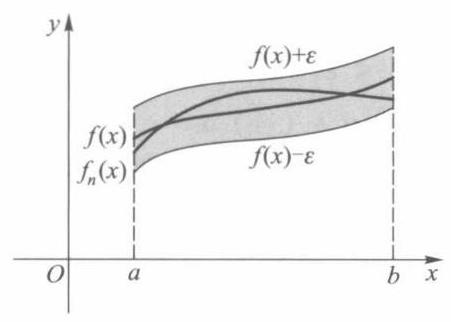
\includegraphics[width=.3\textwidth]{images/P099.jpg}
	\caption{图 $13-1$}
	\label{fig:P099}
\end{figure}

\begin{figure}
	\centering
	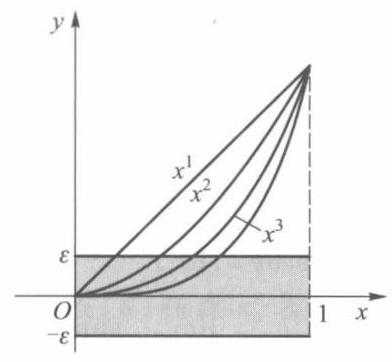
\includegraphics[width=.3\textwidth]{images/P100.jpg}
	\caption{图 $13-2$}
	\label{fig:P100}
\end{figure}

%定理 13.1
\begin{theorem}{}{the:}

\end{theorem}
 (函数列一致收敛的柯西准则) 函数列 \(\left\{  {f}_{n}\right\}\) 在数集 \(D\) 上一致收敛的充要条件是: 对任给正数 \(\varepsilon\) ,总存在正数 \(N\) ,使得当 \(n,m > N\) 时,对一切 \(x \in  D\) ,都有
\[
\left| {{f}_{n}\left( x\right)  - {f}_{m}\left( x\right) }\right|  < \varepsilon . \tag{4}
\]
%证
\begin{proof}

\end{proof}
[必要性] 设 \({f}_{n}\left( x\right)  \rightarrow  f\left( x\right) \left( {n \rightarrow  \infty }\right) ,x \in  D\) ,即对任给 \(\varepsilon  > 0\) ,存在正数 \(N\) ,使得当 \(n > N\) 时,对一切 \(x \in  D\) ,都有
\[
\left| {{f}_{n}\left( x\right)  - f\left( x\right) }\right|  < \frac{\varepsilon }{2}. \tag{5}
\]
于是当 \(n,m > N\) ,由 (5) 就有
\[
\left| {{f}_{n}\left( x\right)  - {f}_{m}\left( x\right) }\right|  \leq  \left| {{f}_{n}\left( x\right)  - f\left( x\right) }\right|  + \left| {f\left( x\right)  - {f}_{m}\left( x\right) }\right|
\]
\[
< \frac{\varepsilon }{2} + \frac{\varepsilon }{2} = \varepsilon \text{ . }
\]
[充分性] 若条件 (4) 成立,由数列收敛的柯西准则, \(\left\{  {f}_{n}\right\}\) 在 \(D\) 上任一点都收敛, 记其极限函数为 \(f\left( x\right) ,x \in  D\) . 现固定 (4) 式中的 \(n\) ,让 \(m \rightarrow  \infty\) ,于是当 \(n > N\) 时,对一切 \(x \in  D\) ,都有
\[
\left| {{f}_{n}\left( x\right)  - f\left( x\right) }\right|  \leq  \varepsilon .
\]
由定义 \(1,{f}_{n}\left( x\right)  \rightarrow  f\left( x\right) \left( {n \rightarrow  \infty }\right) ,x \in  D\) .

根据一致收敛定义可推出下述定理.

%定理 13.2
\begin{theorem}{}{the:}

\end{theorem}
 函数列 \(\left\{  {f}_{n}\right\}\) 在区间 \(D\) 上一致收敛于 \(f\) 的充要条件是:
\[
\mathop{\lim }\limits_{{n \rightarrow  \infty }}\mathop{\sup }\limits_{{x \in  D}}\left| {{f}_{n}\left( x\right)  - f\left( x\right) }\right|  = 0. \tag{6}
\]
%证
\begin{proof}

\end{proof}
[必要性] 若 \({f}_{n}\left( x\right)  \rightarrow  f\left( x\right) \left( {n \rightarrow  \infty }\right) ,x \in  D\) . 则对任给的正数 \(\varepsilon\) ,存在不依赖于 \(x\) 的正整数 \(N\) ,当 \(n > N\) 时,有
\[
\left| {{f}_{n}\left( x\right)  - f\left( x\right) }\right|  < \varepsilon ,\;x \in  D.
\]
由上确界的定义, 亦有
\[
\mathop{\sup }\limits_{{x \in  D}}\left| {{f}_{n}\left( x\right)  - f\left( x\right) }\right|  \leq  \varepsilon .
\]
这就证得 (6) 式成立.

[充分性] 由假设,对任给 \(\varepsilon  > 0\) ,存在正整数 \(N\) ,使得当 \(n > N\) 时,有
\[
\mathop{\sup }\limits_{{x \in  D}}\left| {{f}_{n}\left( x\right)  - f\left( x\right) }\right|  < \varepsilon . \tag{7}
\]
因为对一切 \(x \in  D\) ,总有
\[
\left| {{f}_{n}\left( x\right)  - f\left( x\right) }\right|  \leq  \mathop{\sup }\limits_{{x \in  D}}\left| {{f}_{n}\left( x\right)  - f\left( x\right) }\right| ,
\]
故由(7)式得
\[
\left| {{f}_{n}\left( x\right)  - f\left( x\right) }\right|  < \varepsilon .
\]
于是 \(\left\{  {f}_{n}\right\}\) 在 \(D\) 上一致收敛于 \(f\) .

在判断函数列是否一致收敛上定理 13.2 更为方便一些 (其缺点是必须事先知道它的极限函数),如例 2 ,由于
\[
\mathop{\lim }\limits_{{n \rightarrow  \infty }}\mathop{\sup }\limits_{{x \in  \left( {-\infty , + \infty }\right) }}\left| {\frac{\sin {nx}}{n} - 0}\right|  = \mathop{\lim }\limits_{{n \rightarrow  \infty }}\frac{1}{n} = 0,
\]
所以在 \(\left( {-\infty , + \infty }\right)\) 上, \(\frac{\sin {nx}}{n} \rightarrow  0\left( {n \rightarrow  \infty }\right)\) .

推论 函数列 \(\left\{  {f}_{n}\right\}\) 在 \(D\) 上不一致收敛于 \(f\) 的充分且必要条件是: 存在 \(\left\{  {x}_{n}\right\}   \subset  D\) ,使得 \(\left\{  {{f}_{n}\left( {x}_{n}\right)  - f\left( {x}_{n}\right) }\right\}\) 不收敛于 0 .

%例 3
\begin{example}

\end{example}
设 \({f}_{n}\left( x\right)  = {nx}{\mathrm{e}}^{-n{x}^{2}},x \in  D = \left( {0, + \infty }\right) ,n = 1,2,\cdots\) . 判别 \(\left\{  {{f}_{n}\left( x\right) }\right\}\) 在 \(D\) 上的一致收敛性.

%解
\begin{solution}

\end{solution}
对任意 \(x \in  \left( {0, + \infty }\right) ,\mathop{\lim }\limits_{{n \rightarrow  \infty }}{nx}{\mathrm{e}}^{-n{x}^{2}} = 0 = f\left( x\right)\) . 在 \(\left( {0, + \infty }\right)\) 上,每个 \({nx}{\mathrm{e}}^{-n{x}^{2}}\) 只有一个极大值点 \({x}_{n} = \frac{1}{\sqrt{2n}}\) ,而 \(\mathop{\sup }\limits_{{x \in  \left( {0, + \infty }\right) }}\left| {{f}_{n}\left( x\right) }\right|  = {f}_{n}\left( {x}_{n}\right)  = \sqrt{\frac{n}{2}}{\mathrm{e}}^{-\frac{1}{2}} \rightarrow\)  \(\infty\) . 因此由定理 13.2 可知 \(\left\{  {f}_{n}\right\}\) 在 \(D\) 上不一致收敛于 \(f\) . (见图 13-3)

\begin{figure}
	\centering
	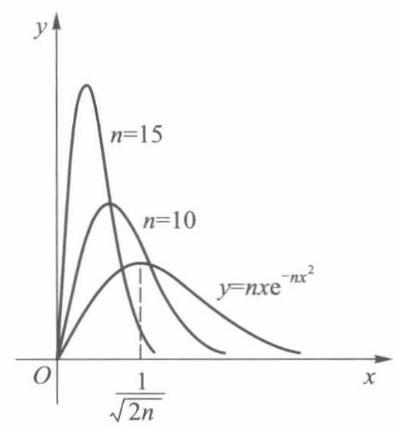
\includegraphics[width=.3\textwidth]{images/P101.jpg}
	\caption{图 $13-3$}
	\label{fig:P101}
\end{figure}

为避免求上确界,亦可取 \({x}_{n} = \frac{1}{n} \in  \left( {0, + \infty }\right)\) ,则 \({f}_{n}\left( {x}_{n}\right)  = {\mathrm{e}}^{-\frac{1}{n}} \rightarrow  1 \neq  0\left( {n \rightarrow  \infty }\right)\) ,因此由推论同样可知 \(\left\{  {f}_{n}\right\}\) 在 \(\left( {0, + \infty }\right)\) 上不一致收敛于 \(f\left( x\right)\) .

%定义  2
\begin{definition}{}{def:}

\end{definition}
设函数列 \(\left\{  {f}_{n}\right\}\) 与 \(f\) 定义在区间 \(I\) 上,若对任意闭区间 \(\left\lbrack  {a,b}\right\rbrack   \subset  I,\left\{  {f}_{n}\right\}\) 在 \(\left\lbrack  {a,b}\right\rbrack\) 上一致收敛于 \(f\) ,则称 \(\left\{  {f}_{n}\right\}\) 在 \(I\) 上内闭一致收敛于 \(f\) .

%注
\begin{remark}

\end{remark}
若 \(I = \left\lbrack  {\alpha ,\beta }\right\rbrack\) 是有界闭区间,显然 \(\left\{  {f}_{n}\right\}\) 在 \(I\) 上内闭一致收敛于 \(f\) 与 \(\left\{  {f}_{n}\right\}\) 在 \(I\) 上一致收敛于 \(f\) 是一致的.

%例 1
\begin{example}

\end{example}
中函数列 \(\left\{  {f}_{n}\right\}\) 在 \(\lbrack 0,1)\) 上不一致收敛于 \(f\) ,但对任意 \(\delta  > 0,\mathop{\sup }\limits_{{x \in  \left\lbrack  {0,\delta }\right\rbrack  }}\left| {x}^{n}\right|  \leq  {\delta }^{n} \rightarrow\)  \(0\left( {n \rightarrow  \infty }\right)\) ,因此 \(\left\{  {f}_{n}\right\}\) 在 \(\lbrack 0,1)\) 上内闭一致收敛.

%例 3
\begin{example}

\end{example}
中函数列 \(\left\{  {f}_{n}\right\}\) 在 \(\left( {0, + \infty }\right)\) 上不一致收敛于 0,但对任意 \(\left\lbrack  {a,b}\right\rbrack   \subset  \left( {0, + \infty }\right)\) , \(\mathop{\sup }\limits_{{x \in  \left\lbrack  {a,b}\right\rbrack  }}\left| {{nx}{\mathrm{e}}^{-n{x}^{2}}}\right|  \leq  {nb}{\mathrm{e}}^{-n{a}^{2}} \rightarrow  0\left( {n \rightarrow  \infty }\right)\) ,因此 \(\left\{  {f}_{n}\right\}\) 在 \(\left( {0, + \infty }\right)\) 上内闭一致收敛于 0 .

\subsection{函数项级数及其一致收敛性}

设 \(\left\{  {{u}_{n}\left( x\right) }\right\}\) 是定义在数集 \(E\) 上的一个函数列,表达式
\[
{u}_{1}\left( x\right)  + {u}_{2}\left( x\right)  + \cdots  + {u}_{n}\left( x\right)  + \cdots ,\;x \in  E \tag{8}
\]
称为定义在 \(E\) 上的函数项级数,简记为 \(\mathop{\sum }\limits_{{n = 1}}^{\infty }{u}_{n}\left( x\right)\) 或 \(\sum {u}_{n}\left( x\right)\) . 称
\[
{S}_{n}\left( x\right)  = \mathop{\sum }\limits_{{k = 1}}^{n}{u}_{k}\left( x\right) ,\;x \in  E,\;n = 1,2,\cdots  \tag{9}
\]
为函数项级数 (8) 的部分和函数列.

若 \({x}_{0} \in  E\) ,数项级数
\[
{u}_{1}\left( {x}_{0}\right)  + {u}_{2}\left( {x}_{0}\right)  + \cdots  + {u}_{n}\left( {x}_{0}\right)  + \cdots  \tag{10}
\]
收敛,即部分和 \({S}_{n}\left( {x}_{0}\right)  = \mathop{\sum }\limits_{{k = 1}}^{n}{u}_{k}\left( {x}_{0}\right)\) 当 \(n \rightarrow  \infty\) 时极限存在,则称级数 (8) 在点 \({x}_{0}\) 收敛, \({x}_{0}\) 称为级数 (8) 的收敛点. 若级数 (10) 发散,则称级数 (8) 在点 \({x}_{0}\) 发散. 若级数 (8) 在 \(E\) 的某个子集 \(D\) 上每点都收敛,则称级数 (8) 在 \(D\) 上收敛. 若 \(D\) 为级数 (8) 全体收敛点的集合,这时则称 \(D\) 为级数 (8) 的收敛域. 级数 (8) 在 \(D\) 上每一点 \(x\) 与其所对应的数项级数 (10) 的和 \(S\left( x\right)\) 构成一个定义在 \(D\) 上的函数,称为级数 (8) 的和函数,并写作
\[
{u}_{1}\left( x\right)  + {u}_{2}\left( x\right)  + \cdots  + {u}_{n}\left( x\right)  + \cdots  = S\left( x\right) ,\;x \in  D,
\]
即
\[
\mathop{\lim }\limits_{{n \rightarrow  \infty }}{S}_{n}\left( x\right)  = S\left( x\right) ,\;x \in  D.
\]
也就是说,函数项级数 (8) 的收敛性就是指它的部分和函数列 (9) 的收敛性.

%例 4
\begin{example}

\end{example}
定义在 \(\left( {-\infty , + \infty }\right)\) 上的函数项级数 (几何级数)
\[
1 + x + {x}^{2} + \cdots  + {x}^{n} + \cdots  \tag{11}
\]
的部分和函数为 \({S}_{n}\left( x\right)  = \frac{1 - {x}^{n}}{1 - x}\) . 当 \(\left| x\right|  < 1\) 时,
\[
S\left( x\right)  = \mathop{\lim }\limits_{{n \rightarrow  \infty }}{S}_{n}\left( x\right)  = \frac{1}{1 - x}.
\]
所以几何级数 (11) 在(-1,1)内收敛于和函数 \(S\left( x\right)  = \frac{1}{1 - x}\) ; 当 \(\left| x\right|  \geq  1\) 时,几何级数是发散的.

%定义  3
\begin{definition}{}{def:}

\end{definition}
设 \(\left\{  {{S}_{n}\left( x\right) }\right\}\) 是函数项级数 \(\sum {u}_{n}\left( x\right)\) 的部分和函数列. 若 \(\left\{  {{S}_{n}\left( x\right) }\right\}\) 在数集 \(D\) 上一致收敛于 \(S\left( x\right)\) ,则称 \(\sum {u}_{n}\left( x\right)\) 在 \(D\) 上一致收敛于 \(S\left( x\right)\) . 若 \(\sum {u}_{n}\left( x\right)\) 在任意闭区间 \(\left\lbrack  {a,b}\right\rbrack   \subset  I\) 上一致收敛,则称 \(\sum {u}_{n}\left( x\right)\) 在 \(I\) 上内闭一致收敛.

由于函数项级数的一致收敛性由它的部分和函数列来确定, 所以由前段中有关函数列一致收敛的定理, 都可推出相应的有关函数项级数的定理.

%定理 13.3
\begin{theorem}{}{the:}

\end{theorem}
 (一致收敛的柯西准则) 函数项级数 \(\sum {u}_{n}\left( x\right)\) 在数集 \(D\) 上一致收敛的充要条件为: 对任给的正数 \(\varepsilon\) ,总存在某正整数 \(N\) ,使得当 \(n > N\) 时,对一切 \(x \in  D\) 和一切正整数 \(p\) ,都有
\[
\left| {{S}_{n + p}\left( x\right)  - {S}_{n}\left( x\right) }\right|  < \varepsilon
\]
或
\[
\left| {{u}_{n + 1}\left( x\right)  + {u}_{n + 2}\left( x\right)  + \cdots  + {u}_{n + p}\left( x\right) }\right|  < \varepsilon .
\]
此定理中当 \(p = 1\) 时,得到函数项级数一致收敛的一个必要条件.

推论 函数项级数 \(\sum {u}_{n}\left( x\right)\) 在数集 \(D\) 上一致收敛的必要条件是函数列 \(\left\{  {{u}_{n}\left( x\right) }\right\}\) 在 \(D\) 上一致收敛于零.

设函数项级数 \(\sum {u}_{n}\left( x\right)\) 在 \(D\) 上的和函数为 \(S\left( x\right)\) ,称
\[
{R}_{n}\left( x\right)  = S\left( x\right)  - {S}_{n}\left( x\right)
\]
为函数项级数 \(\sum {u}_{n}\left( x\right)\) 的余项.

%定理 13.4
\begin{theorem}{}{the:}

\end{theorem}
 函数项级数 \(\sum {u}_{n}\left( x\right)\) 在数集 \(D\) 上一致收敛于 \(S\left( x\right)\) 的充要条件是
\[
\mathop{\lim }\limits_{{n \rightarrow  \infty }}\mathop{\sup }\limits_{{x \in  D}}\left| {{R}_{n}\left( x\right) }\right|  = \mathop{\lim }\limits_{{n \rightarrow  \infty }}\mathop{\sup }\limits_{{x \in  D}}\left| {S\left( x\right)  - {S}_{n}\left( x\right) }\right|  = 0.
\]
我们再来看例 4 中的级数 \(\mathop{\sum }\limits_{{n = 0}}^{\infty }{x}^{n}\) ,由于
\[
\mathop{\sup }\limits_{{x \in  \left( {-1,1}\right) }}\left| {{S}_{n}\left( x\right)  - S\left( x\right) }\right|  = \mathop{\sup }\limits_{{x \in  \left( {-1,1}\right) }}\left| \frac{{x}^{n}}{x - 1}\right|  \geq  \left| \frac{{\left( \frac{n}{n + 1}\right) }^{n}}{1 - \frac{n}{n + 1}}\right|
\]
\[
= n{\left( \frac{n}{n + 1}\right) }^{n - 1} \rightarrow  \infty \;\left( {n \rightarrow  \infty }\right) ,
\]
知道级数 \(\mathop{\sum }\limits_{{n = 0}}^{\infty }{x}^{n}\) 在(-1,1)上不一致收敛.

对任意 \(a\left( {0 < a < 1}\right)\) ,
\[
\mathop{\sup }\limits_{{x \in  \left\lbrack  {-a,a}\right\rbrack  }}\left| {{S}_{n}\left( x\right)  - S\left( x\right) }\right|  = \mathop{\sup }\limits_{{x \in  \left\lbrack  {-a,a}\right\rbrack  }}\left| \frac{-{x}^{n}}{1 - x}\right|  = \frac{{a}^{n}}{1 - a} \rightarrow  0\;\left( {n \rightarrow  \infty }\right)
\]
可得级数 \(\sum {x}^{n}\) 在(-1,1)上内闭一致收敛.

\subsection{函数项级数的一致收敛性判别法}

判别函数项级数的一致收敛性除了根据定义或定理 13.4 外, 有些级数还可根据级数各项的特性来判别.

%定理 13.5
\begin{theorem}{}{the:}

\end{theorem}
 (魏尔斯特拉斯判别法) 设函数项级数 \(\sum {u}_{n}\left( x\right)\) 定义在数集 \(D\) 上, \(\sum {M}_{n}\) 为收敛的正项级数,若对一切 \(x \in  D\) ,有
\[
\left| {{u}_{n}\left( x\right) }\right|  \leq  {M}_{n},\;n = 1,2,\cdots , \tag{12}
\]
则函数项级数 \(\sum {u}_{n}\left( x\right)\) 在 \(D\) 上一致收敛.

%证
\begin{proof}

\end{proof}
由假设正项级数 \(\sum {M}_{n}\) 收敛,根据数项级数的柯西准则,任给正数 \(\varepsilon\) ,存在某正整数 \(N\) ,使得当 \(n > N\) 及任何正整数 \(p\) ,有
\[
\left| {{M}_{n + 1} + \cdots  + {M}_{n + p}}\right|  = {M}_{n + 1} + \cdots  + {M}_{n + p} < \varepsilon .
\]
又由 (12) 式,对一切 \(x \in  D\) 有
\[
\left| {{u}_{n + 1}\left( x\right)  + \cdots  + {u}_{n + p}\left( x\right) }\right|  \leq  \left| {{u}_{n + 1}\left( x\right) }\right|  + \cdots  + \left| {{u}_{n + p}\left( x\right) }\right|
\]
\[
\leq  {M}_{n + 1} + \cdots  + {M}_{n + p} < \varepsilon .
\]
根据函数项级数一致收敛的柯西准则,级数 \(\sum {u}_{n}\left( x\right)\) 在 \(D\) 上一致收敛.

%例 5
\begin{example}

\end{example}
函数项级数
\[
\sum \frac{\sin {nx}}{{n}^{2}},\;\sum \frac{\cos {nx}}{{n}^{2}}
\]
在 \(\left( {-\infty , + \infty }\right)\) 上一致收敛,因为对一切 \(x \in  \left( {-\infty , + \infty }\right)\) 有
\[
\left| \frac{\sin {nx}}{{n}^{2}}\right|  \leq  \frac{1}{{n}^{2}},\;\left| \frac{\cos {nx}}{{n}^{2}}\right|  \leq  \frac{1}{{n}^{2}},
\]
而正项级数 \(\sum \frac{1}{{n}^{2}}\) 是收敛的.

%定理 13.5
\begin{theorem}{}{the:}

\end{theorem}
 也称为 \(\mathbf{M}\) 判别法或优级数判别法. 当级数 \(\sum {u}_{n}\left( x\right)\) 与级数 \(\sum {M}_{n}\) 在区间 \(\left\lbrack  {a,b}\right\rbrack\) 上成立关系式 (12) 时,则称级数 \(\sum {M}_{n}\) 在 \(\left\lbrack  {a,b}\right\rbrack\) 上优于级数 \(\sum {u}_{n}\left( x\right)\) ,或称 \(\sum {M}_{n}\) 为 \(\sum {u}_{n}\left( x\right)\) 的优级数.

下面讨论定义在区间 \(I\) 上形如
\[
\sum {u}_{n}\left( x\right) {v}_{n}\left( x\right)  = {u}_{1}\left( x\right) {v}_{1}\left( x\right)  + {u}_{2}\left( x\right) {v}_{2}\left( x\right)  + \cdots  + {u}_{n}\left( x\right) {v}_{n}\left( x\right)  + \cdots  \tag{13}
\]
的函数项级数的一致收敛性判别法, 它与数项级数一样, 也是基于阿贝尔分部求和公式 (第十二章 §3 的引理).

%定理 13.6
\begin{theorem}{}{the:}

\end{theorem}
(阿贝尔判别法)设

(i) \(\sum {u}_{n}\left( x\right)\) 在区间 \(I\) 上一致收敛;

(ii) 对于每一个 \(x \in  I,\left\{  {{v}_{n}\left( x\right) }\right\}\) 是单调的;

(iii) \(\left\{  {{v}_{n}\left( x\right) }\right\}\) 在 \(I\) 上一致有界,即存在正数 \(M\) ,使得对一切 \(x \in  I\) 和正整数 \(n\) ,有
\[
\left| {{v}_{n}\left( x\right) }\right|  \leq  M,
\]
则级数 (13) 在 \(I\) 上一致收敛.

%证
\begin{proof}

\end{proof}
由 (i),任给 \(\varepsilon  > 0\) ,存在某正数 \(N\) ,使得当 \(n > N\) 及任何正整数 \(p\) ,对一切 \(x \in  I\) ,有
\[
\left| {{u}_{n + 1}\left( x\right)  + \cdots  + {u}_{n + p}\left( x\right) }\right|  < \varepsilon .
\]
又由 (ii), (iii) 及阿贝尔引理 (第十二章 § 3 引理的推论) 得到
\[
\left| {{u}_{n + 1}\left( x\right) {v}_{n + 1}\left( x\right)  + \cdots  + {u}_{n + p}\left( x\right) {v}_{n + p}\left( x\right) }\right|
\]
\[
\leq  \left( {\left| {{v}_{n + 1}\left( x\right) }\right|  + 2\left| {{v}_{n + p}\left( x\right) }\right| }\right) \varepsilon  \leq  {3M\varepsilon }.
\]
于是根据函数项级数一致收敛性的柯西准则就得到本定理的结论.

%定理 13.7
\begin{theorem}{}{the:}

\end{theorem}
(狄利克雷判别法) 设

(i) \(\sum {u}_{n}\left( x\right)\) 的部分和函数列
\[
{S}_{n}\left( x\right)  = \mathop{\sum }\limits_{{k = 1}}^{n}{u}_{k}\left( x\right) \;\left( {n = 1,2,\cdots }\right)
\]
在 \(I\) 上一致有界;

(ii) 对于每一个 \(x \in  I,\left\{  {{v}_{n}\left( x\right) }\right\}\) 是单调的;

(iii) 在 \(I\) 上 \({v}_{n}\left( x\right)  \rightarrow  0\left( {n \rightarrow  \infty }\right)\) ,

则级数 (13) 在 \(I\) 上一致收敛.

%证
\begin{proof}

\end{proof}
证法与定理 13.6 相仿. 由 (i),存在正数 \(M\) ,对一切 \(x \in  I\) ,有 \(\left| {{S}_{n}\left( x\right) }\right|  \leq  M\) . 因此当 \(n,p\) 为任何正整数时,
\[
\left| {{u}_{n + 1}\left( x\right)  + \cdots  + {u}_{n + p}\left( x\right) }\right|  = \left| {{S}_{n + p}\left( x\right)  - {S}_{n}\left( x\right) }\right|  \leq  {2M}.
\]
对任何一个 \(x \in  I\) ,再由 (ii) 及阿贝尔引理,得到
\[
\left| {{u}_{n + 1}\left( x\right) {v}_{n + 1}\left( x\right)  + \cdots  + {u}_{n + p}\left( x\right) {v}_{n + p}\left( x\right) }\right|
\]
\[
\leq  {2M}\left( {\left| {{v}_{n + 1}\left( x\right) }\right|  + 2\left| {{v}_{n + p}\left( x\right) }\right| }\right) .
\]
再由 (iii),对任给的 \(\varepsilon  > 0\) ,存在正数 \(N\) ,当 \(n > N\) 时,对一切 \(x \in  I\) ,有
\[
\left| {{v}_{n}\left( x\right) }\right|  < \varepsilon ,
\]
所以
\[
\left| {{u}_{n + 1}\left( x\right) {v}_{n + 1}\left( x\right)  + \cdots  + {u}_{n + p}\left( x\right) {v}_{n + p}\left( x\right) }\right|  < {2M}\left( {\varepsilon  + {2\varepsilon }}\right)  = {6M\varepsilon }.
\]
于是由一致收敛性的柯西准则,级数 (13) 在 \(I\) 上一致收敛.

%例 6
\begin{example}

\end{example}
函数项级数
\[
\sum \frac{{\left( -1\right) }^{n}{\left( x + n\right) }^{n}}{{n}^{n + 1}}
\]
在 \(\left\lbrack  {0,1}\right\rbrack\) 上一致收敛. 这是因为记 \({u}_{n}\left( x\right)  = \frac{{\left( -1\right) }^{n}}{n},{v}_{n}\left( x\right)  = {\left( 1 + \frac{x}{n}\right) }^{n}\) 时,由阿贝尔判别法 (定理 13.6 ) 就能得到结果.

%例 7
\begin{example}

\end{example}
若数列 \(\left\{  {a}_{n}\right\}\) 单调且收敛于零,则级数
\[
\sum {a}_{n}\cos {nx} \tag{14}
\]
在 \(\left\lbrack  {\alpha ,{2\pi } - \alpha }\right\rbrack  \left( {0 < \alpha  < \pi }\right)\) 上一致收敛.

%证
\begin{proof}

\end{proof}
由第十二章 \(§3\left( {21}\right)\) 式,在 \(\left\lbrack  {\alpha ,{2\pi } - \alpha }\right\rbrack\) 上有
\[
\left| {\mathop{\sum }\limits_{{k = 1}}^{n}\cos {kx}}\right|  = \left| {\frac{\sin \left( {n + \frac{1}{2}}\right) x}{2\sin \frac{x}{2}} - \frac{1}{2}}\right|
\]
\[
\leq  \frac{1}{2\left| {\sin \frac{x}{2}}\right| } + \frac{1}{2} \leq  \frac{1}{2\sin \frac{\alpha }{2}} + \frac{1}{2},
\]
所以级数 \(\sum \cos {nx}\) 的部分和函数列在 \(\left\lbrack  {\alpha ,{2\pi } - \alpha }\right\rbrack\) 上一致有界,于是令
\[
{u}_{n}\left( x\right)  = \cos {nx},{v}_{n}\left( x\right)  = {a}_{n},
\]
则由狄利克雷判别法可得级数 (14) 在 \(\left\lbrack  {\alpha ,{2\pi } - \alpha }\right\rbrack\) 上一致收敛.

对于例 7 中的级数 (14),只要 \(\left\{  {a}_{n}\right\}\) 单调且收敛于零,那么级数 (14) 在不包含 \({2k\pi }\)  \(\left( {k = 0, \pm  1, \pm  2,\cdots }\right)\) 的任何闭区间上都一致收敛.

\subsection{习题 13.1}

1. 讨论下列函数列在所示区间 \(D\) 上是否一致收敛或内闭一致收敛,并说明理由:

(1) \({f}_{n}\left( x\right)  = \sqrt{{x}^{2} + \frac{1}{{n}^{2}}},\;n = 1,2,\cdots ,\;D = \left( {-1,1}\right)\) ;

(2) \({f}_{n}\left( x\right)  = \frac{x}{1 + {n}^{2}{x}^{2}},\;n = 1,2,\cdots ,\;D = \left( {-\infty , + \infty }\right)\) ；

(3) \({f}_{n}\left( x\right)  = \left\{  \begin{array}{ll}  - \left( {n + 1}\right) x + 1, & 0 \leq  x \leq  \frac{1}{n + 1}, \\  0, & \frac{1}{n + 1} < x < 1,\;n = 1,2,\cdots ; \end{array}\right.\)

(4) \({f}_{n}\left( x\right)  = \frac{x}{n},\;n = 1,2,\cdots ,\;D = \lbrack 0, + \infty )\) ；

(5) \({f}_{n}\left( x\right)  = \sin \frac{x}{n},\;n = 1,2,\cdots ,\;D = \left( {-\infty , + \infty }\right)\) .

2. 证明: 设 \({f}_{n}\left( x\right)  \rightarrow  f\left( x\right) ,x \in  D,{a}_{n} \rightarrow  0\left( {n \rightarrow  \infty }\right) \left( {{a}_{n} > 0}\right)\) . 若对每一个正整数 \(n\) 有 \(\left| {{f}_{n}\left( x\right)  - f\left( x\right) }\right|  \leq  {a}_{n},x \in  D\) ,则 \(\left\{  {f}_{n}\right\}\) 在 \(D\) 上一致收敛于 \(f\) .

3. 判别下列函数项级数在所示区间上的一致收敛性:

(1) \(\sum \frac{{x}^{n}}{\left( {n - 1}\right) !},x \in  \left\lbrack  {-r,r}\right\rbrack\) ;

(2) \(\sum \frac{{\left( -1\right) }^{n - 1}{x}^{2}}{{\left( 1 + {x}^{2}\right) }^{n}},x \in  \left( {-\infty , + \infty }\right)\) ；

(3) \(\sum \frac{n}{{x}^{n}},\left| x\right|  > r \geq  1\) ;

(4) \(\sum \frac{{x}^{n}}{{n}^{2}},x \in  \left\lbrack  {0,1}\right\rbrack\) ;

(5) \(\sum \frac{{\left( -1\right) }^{n - 1}}{{x}^{2} + n},x \in  \left( {-\infty , + \infty }\right)\) ;

(6) \(\sum \frac{{x}^{2}}{{\left( 1 + {x}^{2}\right) }^{n - 1}},x \in  \left( {-\infty , + \infty }\right)\) .

4. 设函数项级数 \(\sum {u}_{n}\left( x\right)\) 在 \(D\) 上一致收敛于 \(S\left( x\right)\) ,函数 \(g\left( x\right)\) 在 \(D\) 上有界. 证明级数 \(\sum g\left( x\right) {u}_{n}\left( x\right)\) 在 \(D\) 上一致收敛于 \(g\left( x\right) S\left( x\right)\) .

5. 若在区间 \(I\) 上,对任何正整数 \(n\) ,
\[
\left| {{u}_{n}\left( x\right) }\right|  \leq  {v}_{n}\left( x\right) ,
\]
证明当 \(\sum {v}_{n}\left( x\right)\) 在 \(I\) 上一致收敛时,级数 \(\sum {u}_{n}\left( x\right)\) 在 \(I\) 上也一致收敛.

6. 设 \({u}_{n}\left( x\right) \left( {n = 1,2,\cdots }\right)\) 是 \(\left\lbrack  {a,b}\right\rbrack\) 上的单调函数. 证明: 若 \(\sum {u}_{n}\left( a\right)\) 与 \(\sum {u}_{n}\left( b\right)\) 都绝对收敛,则 \(\sum {u}_{n}\left( x\right)\) 在 \(\left\lbrack  {a,b}\right\rbrack\) 上绝对且一致收敛.

7. 证明: \(\left\{  {f}_{n}\right\}\) 在区间 \(I\) 上内闭一致收敛于 \(f\) 的充分且必要条件是: 对任意 \({x}_{0} \in  I\) ,存在 \({x}_{0}\) 的一个邻域 \(U\left( {x}_{0}\right)\) ,使得 \(\left\{  {f}_{n}\right\}\) 在 \(U\left( {x}_{0}\right)  \cap  I\) 上一致收敛于 \(f\) .

8. 在 \(\left\lbrack  {0,1}\right\rbrack\) 上定义函数列
\[
{u}_{n}\left( x\right)  = \left\{  {\begin{array}{ll} \frac{1}{n}, & x = \frac{1}{n}, \\  0, & x \neq  \frac{1}{n}, \end{array}\;n = 1,2,\cdots ,}\right.
\]
证明级数 \(\sum {u}_{n}\left( x\right)\) 在 \(\left\lbrack  {0,1}\right\rbrack\) 上一致收敛,但它不存在优级数.

9. 讨论下列函数列或函数项级数在所示区间 \(D\) 上的一致收敛性:

(1) \(\mathop{\sum }\limits_{{n = 2}}^{\infty }\frac{1 - {2n}}{\left( {{x}^{2} + {n}^{2}}\right) \left\lbrack  {{x}^{2} + {\left( n - 1\right) }^{2}}\right\rbrack  },D = \left\lbrack  {-1,1}\right\rbrack\) ;

(2) \(\sum {2}^{n}\sin \frac{x}{{3}^{n}},D = \left( {0, + \infty }\right)\) ；

(3) \(\sum \frac{{x}^{2}}{\left\lbrack  {1 + \left( {n - 1}\right) {x}^{2}}\right\rbrack  \left( {1 + n{x}^{2}}\right) },D = \left( {0, + \infty }\right)\) ；

(4) \(\sum \frac{{x}^{n}}{\sqrt{n}},D = \left\lbrack  {-1,0}\right\rbrack\) ;

(5) \(\sum {\left( -1\right) }^{n}\frac{{x}^{{2n} + 1}}{{2n} + 1},D = \left( {-1,1}\right)\) ；

(6) \(\mathop{\sum }\limits_{{n = 1}}^{\infty }\frac{\sin {nx}}{n},D = \left( {0,{2\pi }}\right)\) .

10. 证明: 级数 \(\sum {\left( -1\right) }^{n}{x}^{n}\left( {1 - x}\right)\) 在 \(\left\lbrack  {0,1}\right\rbrack\) 上绝对收敛并一致收敛,但由其各项绝对值组成的级数在 \(\left\lbrack  {0,1}\right\rbrack\) 上却不一致收敛.

11. 设 \(f\) 为定义在区间(a, b)内的任一函数,记
\[
{f}_{n}\left( x\right)  = \frac{\left\lbrack  nf\left( x\right) \right\rbrack  }{n},\;n = 1,2,\cdots ,
\]
证明函数列 \(\left\{  {f}_{n}\right\}\) 在(a, b)内一致收敛于 \(f\) .

12. 设 \(\left\{  {{u}_{n}\left( x\right) }\right\}\) 为 \(\left\lbrack  {a,b}\right\rbrack\) 上正的递减且收敛于零的函数列,每一个 \({u}_{n}\left( x\right)\) 都是 \(\left\lbrack  {a,b}\right\rbrack\) 上的单调函数, 则级数
\[
{u}_{1}\left( x\right)  - {u}_{2}\left( x\right)  + {u}_{3}\left( x\right)  - {u}_{4}\left( x\right)  + \cdots
\]
在 \(\left\lbrack  {a,b}\right\rbrack\) 上不仅收敛,而且一致收敛.

13. 证明: 若 \(\left\{  {{f}_{n}\left( x\right) }\right\}\) 在区间 \(I\) 上一致收敛于 0,则存在子列 \(\left\{  {f}_{{n}_{i}}\right\}\) ,使得 \(\mathop{\sum }\limits_{{i = 1}}^{\infty }{f}_{{n}_{i}}\left( x\right)\) 在 \(I\) 上一致收敛.

\section{一致收敛函数列与函数项级数的性质}

本节讨论由函数列与函数项级数所确定的函数的连续性、可积性与可微性.

%定理 13.8
\begin{theorem}{}{the:}

\end{theorem}
 设函数列 \(\left\{  {f}_{n}\right\}\) 在 \(\left( {a,{x}_{0}}\right)  \cup  \left( {{x}_{0},b}\right)\) 上一致收敛于 \(f\left( x\right)\) ,且对每个 \(n\) , \(\mathop{\lim }\limits_{{x \rightarrow  {x}_{0}}}{f}_{n}\left( x\right)  = {a}_{n}\) ,则 \(\mathop{\lim }\limits_{{n \rightarrow  \infty }}{a}_{n}\) 和 \(\mathop{\lim }\limits_{{x \rightarrow  {x}_{0}}}f\left( x\right)\) 均存在且相等.

%证
\begin{proof}

\end{proof}
先证 \(\left\{  {a}_{n}\right\}\) 是收敛数列. 对任意 \(\varepsilon  > 0\) ,由于 \(\left\{  {f}_{n}\right\}\) 一致收敛,故有 \(N\) ,当 \(n > N\) 时,对任意正整数 \(p\) 和对一切 \(x \in  \left( {a,{x}_{0}}\right)  \cup  \left( {{x}_{0},b}\right)\) ,有
\[
\left| {{f}_{n}\left( x\right)  - {f}_{n + p}\left( x\right) }\right|  < \varepsilon . \tag{1}
\]
从而
\[
\left| {{a}_{n} - {a}_{n + p}}\right|  = \mathop{\lim }\limits_{{x \rightarrow  {x}_{0}}}\left| {{f}_{n}\left( x\right)  - {f}_{n + p}\left( x\right) }\right|  \leq  \varepsilon .
\]
这样由柯西准则可知 \(\left\{  {a}_{n}\right\}\) 是收敛数列.

设 \(\mathop{\lim }\limits_{{n \rightarrow  \infty }}{a}_{n} = A\) . 再证 \(\mathop{\lim }\limits_{{x \rightarrow  {x}_{0}}}f\left( x\right)  = A\) .

由于 \({f}_{n}\left( x\right)\) 一致收敛于 \(f\left( x\right)\) 及 \({a}_{n}\) 收敛于 \(A\) ,因此对任意 \(\varepsilon  > 0\) ,存在正数 \(N\) ,当 \(n > N\) 时,对任意 \(x \in  \left( {a,{x}_{0}}\right)  \cup  \left( {{x}_{0},b}\right)\) ,
\[
\left| {{f}_{n}\left( x\right)  - f\left( x\right) }\right|  < \frac{\varepsilon }{3}\text{ 和 }\left| {{a}_{n} - A}\right|  < \frac{\varepsilon }{3}
\]
同时成立. 特别取 \(n = N + 1\) ,有
\[
\left| {{f}_{N + 1}\left( x\right)  - f\left( x\right) }\right|  < \frac{\varepsilon }{3},\;\left| {{a}_{N + 1} - A}\right|  < \frac{\varepsilon }{3}.
\]
又 \(\mathop{\lim }\limits_{{x \rightarrow  {x}_{0}}}{f}_{N + 1}\left( x\right)  = {a}_{N + 1}\) ,故存在 \(\delta  > 0\) ,当 \(0 < \left| {x - {x}_{0}}\right|  < \delta\) 时,
\[
\left| {{f}_{N + 1}\left( x\right)  - {a}_{N + 1}}\right|  < \frac{\varepsilon }{3}.
\]
这样,当 \(x\) 满足 \(0 < \left| {x - {x}_{0}}\right|  < \delta\) 时,
\[
\left| {f\left( x\right)  - A}\right|  \leq  \left| {f\left( x\right)  - {f}_{N + 1}\left( x\right) }\right|  + \left| {{f}_{N + 1}\left( x\right)  - {a}_{N + 1}}\right|  + \left| {{a}_{N + 1} - A}\right|
\]
\[
< \frac{\varepsilon }{3} + \frac{\varepsilon }{3} + \frac{\varepsilon }{3} = \varepsilon ,
\]
即 \(\mathop{\lim }\limits_{{x \rightarrow  {x}_{0}}}f\left( x\right)  = A\) .

这个定理指出: 在一致收敛的条件下, \(\left\{  {{f}_{n}\left( x\right) }\right\}\) 中两个独立变量 \(x\) 与 \(n\) ,在分别求极限时其求极限的顺序可以交换, 即
\[
\mathop{\lim }\limits_{{x \rightarrow  {x}_{0}}}\mathop{\lim }\limits_{{n \rightarrow  \infty }}{f}_{n}\left( x\right)  = \mathop{\lim }\limits_{{n \rightarrow  \infty }}\mathop{\lim }\limits_{{x \rightarrow  {x}_{0}}}{f}_{n}\left( x\right) . \tag{2}
\]
类似地,若 \({f}_{n}\left( x\right)\) 在(a, b)上一致收敛且 \(\mathop{\lim }\limits_{{x \rightarrow  {a}^{ + }}}{f}_{n}\left( x\right)\) 存在,可推得 \(\mathop{\lim }\limits_{{x \rightarrow  {a}^{ + }}}\mathop{\lim }\limits_{{n \rightarrow  \infty }}{f}_{n}\left( x\right)  =\)  \(\mathop{\lim }\limits_{{n \rightarrow  \infty }}\mathop{\lim }\limits_{{x \rightarrow  {a}^{ + }}}{f}_{n}\left( x\right)\) ; 若 \({f}_{n}\left( x\right)\) 在(a, b)上一致收敛且 \(\mathop{\lim }\limits_{{x \rightarrow  {b}^{ - }}}{f}_{n}\left( x\right)\) 存在,则可推得 \(\mathop{\lim }\limits_{{x \rightarrow  {b}^{ - }}}\mathop{\lim }\limits_{{n \rightarrow  \infty }}{f}_{n}\left( x\right)  =\)  \(\mathop{\lim }\limits_{{n \rightarrow  \infty }}\mathop{\lim }\limits_{{x \rightarrow  {b}^{ - }}}{f}_{n}\left( x\right) .\)

由定理 13.8 可得到以下定理.

%定理 13.9
\begin{theorem}{}{the:}

\end{theorem}
 (连续性) 若函数列 \(\left\{  {f}_{n}\right\}\) 在区间 \(I\) 上一致收敛,且每一项都连续,则其极限函数 \(f\) 在 \(I\) 上也连续.

%证
\begin{proof}

\end{proof}
设 \({x}_{0}\) 为 \(I\) 上任一点. 由于 \(\mathop{\lim }\limits_{{x \rightarrow  {x}_{0}}}{f}_{n}\left( x\right)  = {f}_{n}\left( {x}_{0}\right)\) ,于是由定理 13.8 知 \(\mathop{\lim }\limits_{{x \rightarrow  {x}_{0}}}f\left( x\right)\) 亦存在,且 \(\mathop{\lim }\limits_{{x \rightarrow  {x}_{0}}}f\left( x\right)  = \mathop{\lim }\limits_{{n \rightarrow  \infty }}{f}_{n}\left( {x}_{0}\right)  = f\left( {x}_{0}\right)\) ,因此 \(f\left( x\right)\) 在 \({x}_{0}\) 上连续.

由定理 13.9 可知: 若各项为连续函数的函数列在区间 \(I\) 上其极限函数不连续,则此函数列在区间 \(I\) 上不一致收敛.

例如: 函数列 \(\left\{  {x}^{n}\right\}\) 的各项在 \(( - 1,1\rbrack\) 上都是连续的,但其极限函数
\[
f\left( x\right)  = \left\{  \begin{array}{ll} 0, &  - 1 < x < 1, \\  1, & x = 1 \end{array}\right.
\]
在 \(x = 1\) 时不连续,从而推得 \(\left\{  {x}^{n}\right\}\) 在 \(( - 1,1\rbrack\) 上不一致收敛.

注意到函数 \(f\left( x\right)\) 在 \(x\) 上连续仅与它在 \(x\) 的近旁的性质有关,因此由定理 13.9 可得以下推论.

推论 若连续函数列 \(\left\{  {f}_{n}\right\}\) 在区间 \(I\) 上内闭一致收敛于 \(f\) ,则 \(f\) 在 \(I\) 上连续.

上节例 1 中 \(\left\{  {{f}_{n}\left( x\right) }\right\}   = \left\{  {x}^{n}\right\}\) 在(-1,1)上不一致收敛,但内闭一致收敛,其极限函数在(-1,1)上连续.

%定理 13.10
\begin{theorem}{}{the:}

\end{theorem}
 (可积性) 若函数列 \(\left\{  {f}_{n}\right\}\) 在 \(\left\lbrack  {a,b}\right\rbrack\) 上一致收敛,且每一项都连续,则
\[
{\int }_{a}^{b}\mathop{\lim }\limits_{{n \rightarrow  \infty }}{f}_{n}\left( x\right) \mathrm{d}x = \mathop{\lim }\limits_{{n \rightarrow  \infty }}{\int }_{a}^{b}{f}_{n}\left( x\right) \mathrm{d}x. \tag{3}
\]
%证
\begin{proof}

\end{proof}
设 \(f\) 为函数列 \(\left\{  {f}_{n}\right\}\) 在 \(\left\lbrack  {a,b}\right\rbrack\) 上的极限函数. 由定理 \({13.9},f\) 在 \(\left\lbrack  {a,b}\right\rbrack\) 上连续,从而 \({f}_{n}\left( {n = 1,2,\cdots }\right)\) 与 \(f\) 在 \(\left\lbrack  {a,b}\right\rbrack\) 上都可积.

因为在 \(\left\lbrack  {a,b}\right\rbrack\) 上 \({f}_{n} \rightarrow  f\left( {n \rightarrow  \infty }\right)\) ,故对任给正数 \(\varepsilon\) ,存在 \(N\) ,当 \(n > N\) 时,对一切 \(x \in\)  \(\left\lbrack  {a,b}\right\rbrack\) ,都有
\[
\left| {{f}_{n}\left( x\right)  - f\left( x\right) }\right|  < \varepsilon .
\]
再根据定积分的性质,当 \(n > N\) 时有
\[
\left| {{\int }_{a}^{b}{f}_{n}\left( x\right) \mathrm{d}x - {\int }_{a}^{b}f\left( x\right) \mathrm{d}x}\right|  = \left| {{\int }_{a}^{b}\left( {{f}_{n}\left( x\right)  - f\left( x\right) }\right) \mathrm{d}x}\right|
\]
\[
\leq  {\int }_{a}^{b}\left| {{f}_{n}\left( x\right)  - f\left( x\right) }\right| \mathrm{d}x
\]
\[
\leq  \varepsilon \left( {b - a}\right) \text{ . }
\]
这就证明了等式 (3).

这个定理指出: 在一致收敛的条件下, 极限运算与积分运算的顺序可以交换.

%例 1
\begin{example}

\end{example}
设函数
\[
{f}_{n}\left( x\right)  = \left\{  \begin{array}{ll} {2n}{\alpha }_{n}x, & 0 \leq  x < \frac{1}{2n}, \\  2{\alpha }_{n} - {2n}{\alpha }_{n}x, & \frac{1}{2n} \leq  x < \frac{1}{n},\;n = 1,2,\cdots . \\  0, & \frac{1}{n} \leq  x \leq  1, \end{array}\right.
\]
其图像如图 13-4 所示.

显然 \(\left\{  {{f}_{n}\left( x\right) }\right\}\) 是 \(\left\lbrack  {0,1}\right\rbrack\) 上的连续函数列,且对任意 \(x \in\)  \(\left\lbrack  {0,1}\right\rbrack  ,\mathop{\lim }\limits_{{n \rightarrow  \infty }}{f}_{n}\left( x\right)  = 0\) . 又 \(\mathop{\sup }\limits_{{x \in  \left\lbrack  {0,1}\right\rbrack  }}\left| {{f}_{n}\left( x\right)  - 0}\right|  = {\alpha }_{n}\) ,因此 \(\left\{  {{f}_{n}\left( x\right) }\right\}\) 在 \(\left\lbrack  {0,1}\right\rbrack\) 上一致收敛于 0 的充要条件是 \({\alpha }_{n} \rightarrow  0\left( {n \rightarrow  \infty }\right)\) .

\begin{figure}
	\centering
	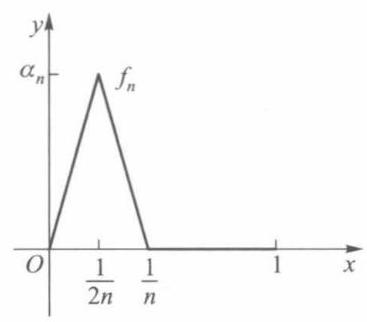
\includegraphics[width=.3\textwidth]{images/P102.jpg}
	\caption{图 $13-4$}
	\label{fig:P102}
\end{figure}

由于 \({\int }_{0}^{1}{f}_{n}\left( x\right) \mathrm{d}x = \frac{{\alpha }_{n}}{2n}\) ,因此 \({\int }_{0}^{1}{f}_{n}\left( x\right) \mathrm{d}x \rightarrow  {\int }_{0}^{1}f\left( x\right) \mathrm{d}x = 0\) 的充要条件是 \(\mathop{\lim }\limits_{{n \rightarrow  \infty }}\frac{{\alpha }_{n}}{2n} = 0\) . 这样当 \({\alpha }_{n} \equiv  1\) 时,虽然 \(\left\{  {{f}_{n}\left( x\right) }\right\}\) 不一致收敛于 \(f\left( x\right)\) ,但定理 13.10 的结论仍成立. 但当 \({\alpha }_{n} = n\) 时, \(\left\{  {{f}_{n}\left( x\right) }\right\}\) 不一致收敛于 \(f\left( x\right)\) ,且 \({\int }_{0}^{1}{f}_{n}\left( x\right) \mathrm{d}x \equiv  \frac{1}{2}\) 也不收敛于 \({\int }_{0}^{1}f\left( x\right) \mathrm{d}x = 0\) .

%例 1
\begin{example}

\end{example}
说明当 \(\left\{  {{f}_{n}\left( x\right) }\right\}\) 收敛于 \(f\left( x\right)\) 时,一致收敛性是极限运算与积分运算交换的充分条件, 但不是必要条件.

%定理 13.11
\begin{theorem}{}{the:}

\end{theorem}
 (可微性) 设 \(\left\{  {f}_{n}\right\}\) 为定义在 \(\left\lbrack  {a,b}\right\rbrack\) 上的函数列,若 \({x}_{0} \in  \left\lbrack  {a,b}\right\rbrack\) 为 \(\left\{  {f}_{n}\right\}\) 的收敛点, \(\left\{  {f}_{n}\right\}\) 的每一项在 \(\left\lbrack  {a,b}\right\rbrack\) 上有连续的导数,且 \(\left\{  {f}^{\prime }\right\}\) 在 \(\left\lbrack  {a,b}\right\rbrack\) 上一致收敛,则
\[
\frac{\mathrm{d}}{\mathrm{d}x}\left( {\mathop{\lim }\limits_{{n \rightarrow  \infty }}{f}_{n}\left( x\right) }\right)  = \mathop{\lim }\limits_{{n \rightarrow  \infty }}\frac{\mathrm{d}}{\mathrm{d}x}{f}_{n}\left( x\right) . \tag{4}
\]
%证
\begin{proof}

\end{proof}
设 \({f}_{n}\left( {x}_{0}\right)  \rightarrow  A\left( {n \rightarrow  \infty }\right) ,{f}_{n}^{\prime }\overrightarrow{ \rightarrow  }g\left( {n \rightarrow  \infty }\right) ,x \in  \left\lbrack  {a,b}\right\rbrack\) . 我们要证明函数列 \(\left\{  {f}_{n}\right\}\) 在区间 \(\left\lbrack  {a,b}\right\rbrack\) 上收敛,且其极限函数的导数存在且等于 \(g\) .

由定理条件,对任一 \(x \in  \left\lbrack  {a,b}\right\rbrack\) ,总有
\[
{f}_{n}\left( x\right)  = {f}_{n}\left( {x}_{0}\right)  + {\int }_{{x}_{0}}^{x}{f}_{n}^{\prime }\left( t\right) \mathrm{d}t.
\]
当 \(n \rightarrow  \infty\) 时,右边第一项极限为 \(A\) ,第二项极限为 \({\int }_{{x}_{0}}^{x}g\left( t\right) \mathrm{d}t\) (定理 13.10),所以左边极限存在,记为 \(f\) ,则有
\[
f\left( x\right)  = \mathop{\lim }\limits_{{n \rightarrow  \infty }}{f}_{n}\left( x\right)  = f\left( {x}_{0}\right)  + {\int }_{{x}_{0}}^{x}g\left( t\right) \mathrm{d}t,
\]
其中 \(f\left( {x}_{0}\right)  = A\) . 由 \(g\) 的连续性及微积分学基本定理 (第九章 §5 ) 推得
\[
{f}^{\prime } = g\text{ . }
\]
这就证明了等式(4).

在定理 13.11 的条件下,还可推出在 \(\left\lbrack  {a,b}\right\rbrack\) 上 \({f}_{n} \rightarrow  f\left( {n \rightarrow  \infty }\right)\) ,请读者自己证明.

由于函数的可微性是函数的局部性质, 故以下推论成立.

推论 设函数列 \(\left\{  {f}_{n}\right\}\) 定义在区间 \(I\) 上,若 \({x}_{0} \in  I\) 为 \(\left\{  {f}_{n}\right\}\) 的收敛点,且 \(\left\{  {f}_{n}^{\prime }\right\}\) 在 \(I\) 上内闭一致收敛,则 \(f\) 在 \(I\) 上可导,且 \({f}^{\prime }\left( x\right)  = \mathop{\lim }\limits_{{n \rightarrow  \infty }}{f}_{n}^{\prime }\left( x\right)\) .

%例 2
\begin{example}

\end{example}
函数列
\[
{f}_{n}\left( x\right)  = \frac{1}{2n}\ln \left( {1 + {n}^{2}{x}^{2}}\right) ,\;n = 1,2,\cdots
\]
与
\[
{f}_{n}^{\prime }\left( x\right)  = \frac{nx}{1 + {n}^{2}{x}^{2}},\;n = 1,2,\cdots
\]
在 \(\left\lbrack  {0,1}\right\rbrack\) 上都收敛于 0,由于
\[
\mathop{\lim }\limits_{{n \rightarrow  \infty }}\mathop{\max }\limits_{{x \in  \left\lbrack  {0,1}\right\rbrack  }}\left| {{f}_{n}^{\prime }\left( x\right)  - {f}^{\prime }\left( x\right) }\right|  = \frac{1}{2},
\]
所以导函数列 \(\left\{  {{f}_{n}^{\prime }\left( x\right) }\right\}\) 在 \(\left\lbrack  {0,1}\right\rbrack\) 上不一致收敛,但对任意 \(\delta  > 0\) ,
\[
\mathop{\sup }\limits_{{x \in  \left\lbrack  {\delta ,1}\right\rbrack  }}\left| {{f}_{n}^{\prime }\left( x\right)  - {f}^{\prime }\left( x\right) }\right|  \leq  \frac{n}{1 + {n}^{2}\delta } \rightarrow  0\;\left( {n \rightarrow  \infty }\right) ,
\]
所以 \(\left\{  {f}_{n}^{\prime }\right\}\) 在 \((0,1\rbrack\) 上内闭一致收敛. 由推论,在 \((0,1\rbrack\) 上, \(\mathop{\lim }\limits_{{n \rightarrow  \infty }}{f}_{n}^{\prime }\left( x\right)  = {\left( \mathop{\lim }\limits_{{n \rightarrow  \infty }}{f}_{n}\left( x\right) \right) }^{\prime }\) 仍成立.

事实上, \(\mathop{\lim }\limits_{{n \rightarrow  \infty }}{f}_{n}^{\prime }\left( x\right)  = 0,\mathop{\lim }\limits_{{n \rightarrow  \infty }}{f}_{n}\left( x\right)  = 0,\mathop{\lim }\limits_{{n \rightarrow  \infty }}{f}_{n}^{\prime }\left( x\right)  = {\left( \mathop{\lim }\limits_{{n \rightarrow  \infty }}{f}_{n}\left( x\right) \right) }^{\prime }\) 在 \(\left\lbrack  {0,1}\right\rbrack\) 上都成立.

此例说明, 一致收敛性是极限运算与求导运算交换的充分条件, 而不是必要条件. 现在再来讨论定义在区间 \(\left\lbrack  {a,b}\right\rbrack\) 上函数项级数
\[
{u}_{1}\left( x\right)  + {u}_{2}\left( x\right)  + \cdots  + {u}_{n}\left( x\right)  + \cdots  \tag{5}
\]
的连续性、逐项求积与逐项求导的性质, 这些性质可由函数列的相应性质推出.

%定理 13.12
\begin{theorem}{}{the:}

\end{theorem}
 (连续性) 若函数项级数 \(\sum {u}_{n}\left( x\right)\) 在区间 \(\left\lbrack  {a,b}\right\rbrack\) 上一致收敛,且每一项都连续,则其和函数在 \(\left\lbrack  {a,b}\right\rbrack\) 上也连续.


这个定理指出: 在一致收敛条件下, (无限项) 求和运算与求极限运算可以交换顺序, 即
\[
\sum \left( {\mathop{\lim }\limits_{{x \rightarrow  {x}_{0}}}{u}_{n}\left( x\right) }\right)  = \mathop{\lim }\limits_{{x \rightarrow  {x}_{0}}}\left( {\sum {u}_{n}\left( x\right) }\right) . \tag{6}
\]
%定理 13.13
\begin{theorem}{}{the:}

\end{theorem}
 (逐项求积) 若函数项级数 \(\sum {u}_{n}\left( x\right)\) 在 \(\left\lbrack  {a,b}\right\rbrack\) 上一致收敛,且每一项 \({u}_{n}\left( x\right)\) 都连续,则
\[
\sum {\int }_{a}^{b}{u}_{n}\left( x\right) \mathrm{d}x = {\int }_{a}^{b}\sum {u}_{n}\left( x\right) \mathrm{d}x. \tag{7}
\]
%定理 13.14
\begin{theorem}{}{the:}

\end{theorem}
 (逐项求导) 若函数项级数 \(\sum {u}_{n}\left( x\right)\) 在 \(\left\lbrack  {a,b}\right\rbrack\) 上每一项都有连续的导函数, \({x}_{0} \in  \left\lbrack  {a,b}\right\rbrack\) 为 \(\sum {u}_{n}\left( x\right)\) 的收敛点,且 \(\sum {u}_{n}^{\prime }\left( x\right)\) 在 \(\left\lbrack  {a,b}\right\rbrack\) 上一致收敛,则
\[
\sum \left( {\frac{\mathrm{d}}{\mathrm{d}x}{u}_{n}\left( x\right) }\right)  = \frac{\mathrm{d}}{\mathrm{d}x}\left( {\sum {u}_{n}\left( x\right) }\right) . \tag{8}
\]
%定理 13.13
\begin{theorem}{}{the:}

\end{theorem}
 和定理 13.14 指出, 在一致收敛条件下, 逐项求积或求导后求和等于求和后再求积或求导.

最后, 我们指出, 本节中六个定理的意义不只是检验函数列或函数项级数是否满足关系式 (2) 一 (4) , (6) 一 (8) ,更重要的是根据定理的条件,即使没有求出极限函数或和函数, 也能由函数列或函数项级数本身获得极限函数或和函数的解析性质.

%例 3
\begin{example}

\end{example}
设
\[
{u}_{n}\left( x\right)  = \frac{1}{{n}^{3}}\ln \left( {1 + {n}^{2}{x}^{2}}\right) ,\;n = 1,2,\cdots .
\]
证明函数项级数 \(\sum {u}_{n}\left( x\right)\) 在 \(\left\lbrack  {0,1}\right\rbrack\) 上一致收敛,并讨论其和函数在 \(\left\lbrack  {0,1}\right\rbrack\) 上的连续性、 可积性与可微性.

%证
\begin{proof}

\end{proof}
对每一个 \(n\) ,易见 \({u}_{n}\left( x\right)\) 为 \(\left\lbrack  {0,1}\right\rbrack\) 上增函数,故有
\[
{u}_{n}\left( x\right)  \leq  {u}_{n}\left( 1\right)  = \frac{1}{{n}^{3}}\ln \left( {1 + {n}^{2}}\right) ,\;n = 1,2,\cdots .
\]
又当 \(t \geq  1\) 时,有不等式 \(\ln \left( {1 + {t}^{2}}\right)  < t\) ,所以
\[
{u}_{n}\left( x\right)  \leq  \frac{1}{{n}^{3}}\ln \left( {1 + {n}^{2}}\right)  < \frac{1}{{n}^{3}} \cdot  n = \frac{1}{{n}^{2}},\;n = 1,2,\cdots .
\]
以收敛级数 \(\sum \frac{1}{{n}^{2}}\) 为 \(\sum {u}_{n}\left( x\right)\) 的优级数,推得 \(\sum {u}_{n}\left( x\right)\) 在 \(\left\lbrack  {0,1}\right\rbrack\) 上一致收敛.

由于每一个 \({u}_{n}\left( x\right)\) 在 \(\left\lbrack  {0,1}\right\rbrack\) 上连续,根据定理 13.12 与定理 \({13.13},\sum {u}_{n}\left( x\right)\) 的和函数 \(S\left( x\right)\) 在 \(\left\lbrack  {0,1}\right\rbrack\) 上连续且可积. 又由
\[
{u}_{n}^{\prime }\left( x\right)  = \frac{2x}{n\left( {1 + {n}^{2}{x}^{2}}\right) } = \frac{2nx}{{n}^{2}\left( {1 + {n}^{2}{x}^{2}}\right) } \leq  \frac{1}{{n}^{2}},\;n = 1,2,\cdots ,
\]
即 \(\sum \frac{1}{{n}^{2}}\) 也是 \(\sum {u}_{n}^{\prime }\left( x\right)\) 的优级数,故 \(\sum {u}_{n}^{\prime }\left( x\right)\) 也在 \(\left\lbrack  {0,1}\right\rbrack\) 上一致收敛. 由定理 13.14,得 \(S\left( x\right)\) 在 \(\left\lbrack  {0,1}\right\rbrack\) 上可微.

与函数列的情况相同, 定理 13.12 和定理 13.14 中的一致收敛的条件可以减弱为内闭一致收敛.

%例 4
\begin{example}

\end{example}
证明: 函数 \(\zeta \left( x\right)  = \mathop{\sum }\limits_{{n = 1}}^{\infty }\frac{1}{{n}^{x}}\) 在 \(\left( {1, + \infty }\right)\) 上有连续的各阶导函数.

%证
\begin{proof}

\end{proof}
设 \({u}_{n}\left( x\right)  = \frac{1}{{n}^{x}}\) ,则 \({u}_{n}^{\left( k\right) }\left( x\right)  = {\left( -1\right) }^{k}\frac{{\ln }^{k}n}{{n}^{x}},k = 1,2,\cdots\) . 设 \(\left\lbrack  {a,b}\right\rbrack   \subset  \left( {1, + \infty }\right)\) ,对任意 \(x \in  \left\lbrack  {a,b}\right\rbrack\) ,有
\[
\left| {{u}_{n}^{\left( k\right) }\left( x\right) }\right|  = \frac{{\ln }^{k}n}{{n}^{x}} \leq  \frac{{\ln }^{k}n}{{n}^{a}},\;k = 1,2,\cdots .
\]
由于 \(\mathop{\lim }\limits_{{n \rightarrow  \infty }}\frac{{\ln }^{k}n}{{n}^{\left( {a - 1}\right) /2}} = 0\) ,因此对于充分大的 \(n,\frac{{\ln }^{k}n}{{n}^{\left( {a - 1}\right) /2}} < 1\) ,从而
\[
\frac{{\ln }^{k}n}{{n}^{a}} = \frac{1}{{n}^{\left( {a + 1}\right) /2}} \cdot  \frac{{\ln }^{k}n}{{n}^{\left( {a - 1}\right) /2}} < \frac{1}{{n}^{\left( {a + 1}\right) /2}}.
\]
因为 \(\mathop{\sum }\limits_{{n = 1}}^{\infty }\frac{1}{{n}^{\left( {a + 1}\right) /2}}\) 收敛,所以 \(\mathop{\sum }\limits_{{n = 1}}^{\infty }{u}_{n}^{\left( k\right) }\left( x\right)\) 在 \(\left\lbrack  {a,b}\right\rbrack\) 上一致收敛,于是 \(\mathop{\sum }\limits_{{n = 1}}^{\infty }{u}_{n}^{\left( k\right) }\left( x\right)\) 在 \(\left( {1, + \infty }\right)\) 上内闭一致收敛. 对 \(\mathop{\sum }\limits_{{n = 1}}^{\infty }{\left( -1\right) }^{k}\frac{{\ln }^{k}n}{{n}^{x}}\) 用定理 13.12 和定理 13.14, \(\zeta \left( x\right)\) 在 \(\left( {1, + \infty }\right)\) 上有连续的各阶导函数,且 \({\zeta }^{\left( k\right) }\left( x\right)  = \mathop{\sum }\limits_{{n = 1}}^{\infty }{\left( -1\right) }^{k}\frac{{\ln }^{k}n}{{n}^{x}},k = 1,2,\cdots\) .

\subsection{习题 13.2}

1. 讨论下列各函数列 \(\left\{  {f}_{n}\right\}\) 在所定义的区间上:

(a) \(\left\{  {f}_{n}\right\}\) 与 \(\left\{  {f}_{n}^{\prime }\right\}\) 的一致收敛性;

(b) \(\left\{  {f}_{n}\right\}\) 是否有定理 13.9,13.10,13.11 的条件与结论.

(1) \({f}_{n}\left( x\right)  = \frac{{2x} + n}{x + n},x \in  \left\lbrack  {0,b}\right\rbrack  ;\;\left( 2\right) {f}_{n}\left( x\right)  = x - \frac{{x}^{n}}{n},x \in  \left\lbrack  {0,1}\right\rbrack\) ;

(3) \({f}_{n}\left( x\right)  = {nx}{\mathrm{e}}^{-n{x}^{2}},x \in  \left\lbrack  {0,1}\right\rbrack\) .

2. 证明: 若函数列 \(\left\{  {f}_{n}\right\}\) 在 \(\left\lbrack  {a,b}\right\rbrack\) 上满足定理 13.11 的条件,则 \(\left\{  {f}_{n}\right\}\) 在 \(\left\lbrack  {a,b}\right\rbrack\) 上一致收敛.

3. 证明定理 13.12 和定理 13.14 .

4. 设 \(S\left( x\right)  = \mathop{\sum }\limits_{{n = 1}}^{\infty }\frac{{x}^{n - 1}}{{n}^{2}},x \in  \left\lbrack  {-1,1}\right\rbrack\) ,计算积分 \({\int }_{0}^{x}S\left( t\right) \mathrm{d}t\) .

5. 设 \(S\left( x\right)  = \mathop{\sum }\limits_{{n = 1}}^{\infty }\frac{\cos {nx}}{n\sqrt{n}},x \in  \left( {-\infty , + \infty }\right)\) ,计算积分 \({\int }_{0}^{x}S\left( t\right) \mathrm{d}t\) .

6. 设 \(S\left( x\right)  = \mathop{\sum }\limits_{{n = 1}}^{\infty }n{\mathrm{e}}^{-{nx}},x > 0\) ,计算 \({\int }_{\ln 2}^{\ln 3}S\left( t\right) \mathrm{d}t\) .

7. 证明:函数 \(f\left( x\right)  = \sum \frac{\sin {nx}}{{n}^{3}}\) 在 \(\left( {-\infty , + \infty }\right)\) 上连续,且有连续的导函数.

8. 证明: 定义在 \(\left\lbrack  {0,{2\pi }}\right\rbrack\) 上的函数项级数 \(\mathop{\sum }\limits_{{n = 0}}^{\infty }{r}^{n}\cos {nx}\left( {0 < r < 1}\right)\) 满足定理 13.13 条件,且 \({\int }_{0}^{2\pi }\left( {\mathop{\sum }\limits_{{n = 0}}^{\infty }{r}^{n}\cos {nx}}\right) \mathrm{d}x = {2\pi }.\)

9. 讨论下列函数列在所定义区间上的一致收敛性及极限函数的连续性、可微性和可积性:

(1) \({f}_{n}\left( x\right)  = x{\mathrm{e}}^{-n{x}^{2}},n = 1,2,\cdots ,x \in  \left\lbrack  {-l,l}\right\rbrack\) ;

(2) \({f}_{n}\left( x\right)  = \frac{nx}{{nx} + 1},n = 1,2,\cdots\) , (i) \(x \in  \lbrack 0, + \infty )\) , (ii) \(x \in  \lbrack a, + \infty )\left( {a > 0}\right)\) .

10. 设 \(f\) 在 \(\left( {-\infty , + \infty }\right)\) 上有任意阶导数,记 \({F}_{n} = {f}^{\left( n\right) }\) ,且在任何有限区间内
\[
{F}_{n} \rightarrow  \varphi \left( {n \rightarrow  \infty }\right) ,
\]
试证 \(\varphi \left( x\right)  = c{\mathrm{e}}^{x}\) ( \(c\) 为常数).

\section{总练习题}

1. 试问 \(k\) 为何值时,下列函数列 \(\left\{  {f}_{n}\right\}\) 一致收敛:

(1) \({f}_{n}\left( x\right)  = x{n}^{k}{\mathrm{e}}^{-{nx}},0 \leq  x <  + \infty\) ;

( 2 ) \({f}_{n}\left( x\right)  = \left\{  \begin{array}{ll} x{n}^{k}, & 0 \leq  x \leq  \frac{1}{n}, \\  \left( {\frac{2}{n} - x}\right) {n}^{k}, & \frac{1}{n} < x \leq  \frac{2}{n}, \\  0, & \frac{2}{n} < x \leq  1. \end{array}\right.\)

2. 证明: (1) 若 \({f}_{n}\left( x\right)  \rightarrow  f\left( x\right) \left( {n \rightarrow  \infty }\right) ,x \in  I\) ,且 \(f\) 在 \(I\) 上有界,则 \(\left\{  {f}_{n}\right\}\) 至多除有限项外在 \(I\) 上是一致有界的;

(2) 若 \({f}_{n}\left( x\right)  \rightarrow  f\left( x\right) \left( {n \rightarrow  \infty }\right) ,x \in  I\) ,且对每个正整数 \(n,{f}_{n}\) 在 \(I\) 上有界,则 \(\left\{  {f}_{n}\right\}\) 在 \(I\) 上一致有界.

3. 设 \(f\) 为 \(\left\lbrack  {\frac{1}{2},1}\right\rbrack\) 上的连续函数. 证明:

(1) \(\left\{  {{x}^{n}f\left( x\right) }\right\}\) 在 \(\left\lbrack  {\frac{1}{2},1}\right\rbrack\) 上收敛;

(2) \(\left\{  {{x}^{n}f\left( x\right) }\right\}\) 在 \(\left\lbrack  {\frac{1}{2},1}\right\rbrack\) 上一致收敛的充要条件是 \(f\left( 1\right)  = 0\) .

4. 若把定理 13.10 中一致收敛函数列 \(\left\{  {f}_{n}\right\}\) 的每一项在 \(\left\lbrack  {a,b}\right\rbrack\) 上连续改为在 \(\left\lbrack  {a,b}\right\rbrack\) 上可积,试证 \(\left\{  {f}_{n}\right\}\) 在 \(\left\lbrack  {a,b}\right\rbrack\) 上的极限函数在 \(\left\lbrack  {a,b}\right\rbrack\) 上也可积.

5. 设级数 \(\sum {a}_{n}\) 收敛. 证明
\[
\mathop{\lim }\limits_{{x \rightarrow  {0}^{ + }}}\sum \frac{{a}_{n}}{{n}^{x}} = \sum {a}_{n}.
\]
6. 设可微函数列 \(\left\{  {f}_{n}\right\}\) 在 \(\left\lbrack  {a,b}\right\rbrack\) 上收敛, \(\left\{  {f}_{n}^{\prime }\right\}\) 在 \(\left\lbrack  {a,b}\right\rbrack\) 上一致有界. 证明: \(\left\{  {f}_{n}\right\}\) 在 \(\left\lbrack  {a,b}\right\rbrack\) 上一致收敛.

7. 设连续函数列 \(\left\{  {{f}_{n}\left( x\right) }\right\}\) 在 \(\left\lbrack  {a,b}\right\rbrack\) 上一致收敛于 \(f\left( x\right)\) ,而 \(g\left( x\right)\) 在 \(\left( {-\infty , + \infty }\right)\) 上连续. 证明: \(\left\{  {g\left( {{f}_{n}\left( x\right) }\right) }\right\}\) 在 \(\left\lbrack  {a,b}\right\rbrack\) 上一致收敛于 \(g\left( {f\left( x\right) }\right)\) .


